\section{Auswertung}

Zuerst werden die Werte aus \ref{tab:7a} in einem Diagramm dargestellt.
Dazu werden auch noch Fehlerbalken dargestellt,
welche die Unsicherheit der Messwerte von $\sqrt{N}$ anzeigen.

\noindent Es sieht folgendermaßen aus:

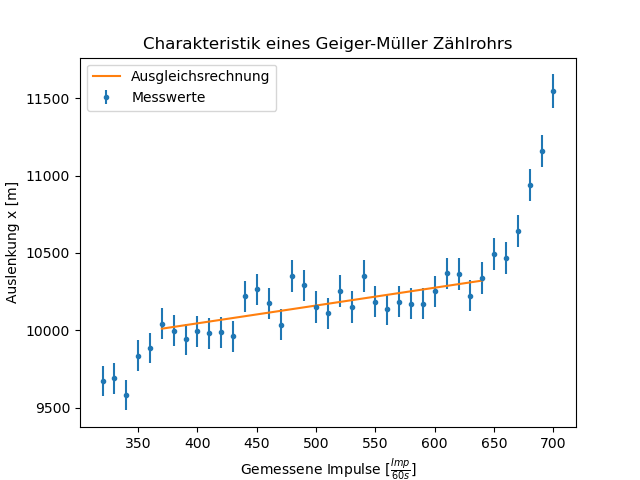
\includegraphics{7a.png}

\subsection{Länge des Plateau-Bereichs}

\noindent In diesem Diagramm ist ein Plateau zu erkennen.
Es erstreckt sich von einer Spannung von 370V bis zu einer Spannung von 640V.
Die Länge dieses Plateau-Bereichs beträgt also 270V.

\subsection{Plateau-Steigung}

Für die Plateau-Steigung wurde eine Ausgleichsrechnung mit der Python-Funktion "$curve_fit$" aus "$scipy.optimize$", im Plateau-Bereich, durchgeführt.
Dafür wurde eine Funktion der folgenden Form verwendet:

\begin{displaymath}
    y = mx + n
\end{displaymath}

\noindent Für die Parameter m und n ergibt sich:

\begin{center}
    \begin{tabular}{ll@{${}\pm{}$}l}
        \toprule
        Parameter & Wert & Unsicherheit\\
        \midrule
        m &    1.151888 & 0.223673 \\
        n &   9584.296388 & 114.390865 \\
        \bottomrule
        
    \end{tabular}
\end{center}

\noindent Dabei ist zu sagen, dass der Parameter m den Wert $\frac{1}{60Vs}$ und der Parameter n die Einheit $\frac{1}{60s}$ hat.

\noindent Die geforderte Plateau-Steigung ergibt sich durch folgende Vorgehensweise:
\begin{align}
     m_{\%} = \frac{N(U_2)-N(U_1)}{N(U_2)}
\end{align}

\noindent Dabei ist $m_{\%}$ die prozentuale Steigung des gesamten Plateaus, 
N ist die Ausgleichsfunktion,
U\textsubscript{1} ist die Spannung, bei der das Plateau beginnt (370 V)
und U\textsubscript{2} ist die Spannung, bei der das Plateau endet (640 V).
Weil das Plateau eine Länge von 270 V hat besitzt $m_{\%}$ die Einheit $\frac{\%}{270V}$.
Deshalb muss $m_{\%}$ noch durch 2,7 geteilt werden um die geforderte Einheit von $\frac{\%}{100V}$ zu erreichen.

\noindent Die Plateau-Steigung in $\frac{\%}{100V}$ hat den Wert:

\begin{displaymath}
    (1.12 \pm 0.2) \frac{\%}{100V}
\end{displaymath}


\subsection{Totzeit}

\noindent Die Totzeit des Zählrohrs lässt sich mit der Zwei-Quellen-Methode durch folgende Formel bestimmen:

\begin{displaymath}
    T = \frac{N_1+N_2-N_{1+2}}{2N_1N_2}
\end{displaymath}

\noindent Mit den Werten:

\begin{align}
    N_1 &= (96041 \pm 309.9048) \frac{1}{120s} = (800.3 \pm 2.6) \frac{1}{s} \nonumber \\
    N_{1+2} &= (158479 \pm 398.0942) \frac{1}{120s} = (1320.7 \pm 3.3) \frac{1}{s} \nonumber \\
    N_2 &= (76518 \pm 276.6189) \frac{1}{120s} = (637.6 \pm 2.3) \frac{1}{s} \nonumber
\end{align}

\noindent ergibt  sich die Totzeit zu $(115 \pm 4)\mu s$.

\noindent Ein weiterer Weg die Totzeit zu bestimmen ist das Ablesen am Oszilloskop.
Dieser Weg liefert eine Totzeit von 100$\mu s$.

\subsection{Freigesetzte Ladungen pro einfallendem Teilchen}

Die Zahl der freigesetzten Ladungen pro einfallendem Teilchen lässt sich mit der folgenden Formel berechnen:

\begin{displaymath}
    Z = \frac{I}{e_0N}
\end{displaymath}

\noindent Bei der Rechnung ergeben sich die Folgenden Werte für Z:

\begin{minipage}{\linewidth}
    \begin{table}[H]
        \centering
    
    \begin{tabular}{ll@{${}\pm{}$}l}
        \toprule
        U [V] & Z [$e^{10}$] & $\Delta$Z [$e^{9}$]\\
        \midrule
        350 & 1.14 & 2.10 \\
        400 & 1.50 & 2.20 \\
        450 & 2.55 & 2.67 \\
        500 & 2.95 & 2.92 \\
        550 & 3.68 & 3.37 \\
        600 & 4.75 & 4.07 \\
        650 & 5.00 & 4.18 \\
        700 & 5.84 & 4.51 \\
        \bottomrule
        
    \end{tabular}
    \captionof{table}{Freigesetzte Ladungen pro einfallendem Teilchen}
    \label{tab:7d}
    \end{table}
\end{minipage}

\noindent Die benötigten Werte stehen in der Tabelle \ref{tab:7d2}.

\noindent Diese Werte werden nun zur Veranschaulichung graphisch dargestellt.
Dafür werden sie gegen die Spannung in einem Diagramm aufgetragen.
Außerdem werden die Unsicherheiten der einzelnen Werte in dem Diagramm als Fehlerbalken dargestellt.
Das entstehende Diagramm ist das Folgende:

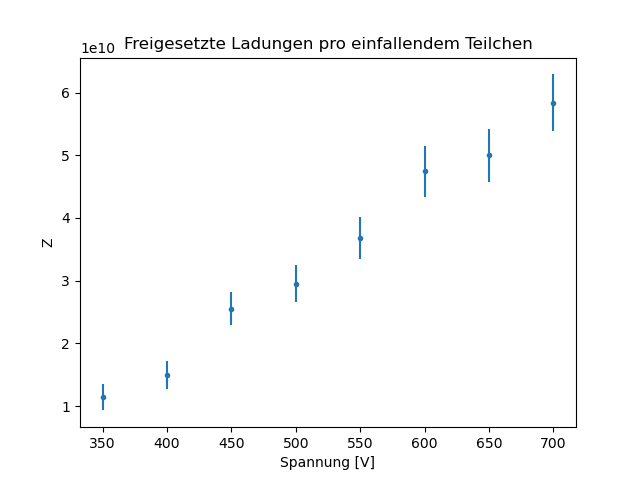
\includegraphics{7d.png}


\section{Diskussion}

\subsection{Länge des Plateau-Bereichs}

Zur Länge des Plateau-Bereichs ist lediglich zu sagen,
dass ein längerer Plateau-Bereich immer besser wäre.
Das liegt daran, dass bei Spannungen,
die außerhalb des Plateau-Bereichs liegen,
entweder nicht richtig funktioniert oder zerstört wird.
Ein Längerer Plateau-Bereich würde also einen größeren Arbeitsbereich des Zählrohrs liefern.
Aufgrund fehlender Vergleichswerte kann an dieser Stelle jedoch keine Aussage darüber getroffen werden,
ob der gemessene Plateau-Bereich nun lang oder kurz ist.

\subsection{Plateau-Steigung}

Ideal wäre hier wenn die Plateau-Steigung = 0 wäre.
Dies ist aber, wie in der Theorie bereits erwähnt,
praktisch nicht umsetzbar,
da sich Nachentladungen nie vollständig vermeiden lassen 
und so immer eine gewisse Steigung entsteht.
Auch sorgen hier gewissen Messfehler eventuell für eine stärkere Steigung.
Die Steigung ist mit 2$\%$ pro 100 Volt aber im realistischen Bereich.
Hier bleibt allerdings nur die Aussage, dass eine Steigung näher an 0 besser wäre,
denn es fehlt ein Vergleichswert um eine genauere Bewertung vorzunehmen.

\subsection{Totzeit}

Bei der Totzeit gilt: Je kleiner diese ist, desto besser.
Die gemessene Totzeit beträgt 115$\mu s$ 
und weist einen sehr geringen Fehler von >4$\%$ auf.
Da die Totzeit sehr kurz und der Fehler gering ist,
scheint die Bestimmung der Totzeit ein Erfolg gewesen zu sein.
Mit dem Oszilloskop ergab sich eine Totzeit von 100$\mu s$.
Dieser Wert weicht von dem durch die Zwei-Quellen-Methode bestimmten Wert um 15\% ab.
Außerdem ist durch das graphische Ablesen am Oszilloskop die Unsicherheit dieses Wertes um ein vielfaches größer.
Die zwei Quellen Methode ist also die wesentlich genauere Methode zur Bestimmung der Totzeit.

\subsection{freigesetzte Ladungen pro einfallendem Teilchen}

Die freigesetzten Ladungen pro einfallendem Teilchen liefern sehr große Werte.
Dies ist zu erklären mit dem Arbeitsbereich des Geiger-Müller Zählrohrs.
Dieser liegt nämlich bei einer Anzahl von Elektronen-Paaren in der Größenordnung von 10 hoch 10.
Damit sind die berechneten Werte im Bereich von 10 hoch 9 bis 10 hoch 10 durchaus im realistischen Bereich.

\subsection{Fazit}

Die Messunsicherheiten bleiben in einem akzeptablen Bereich und damit sind auch die entstehenden Fehler in Rechnungen eher gering.
Dies liegt wahrscheinlich auch an einer Überlegung, die vor dem Experiment im Bezug auf den Aufbau gemacht wurde.
So wurde die verwendete Tl-Quelle so plaziert, 
dass bei einer mittleren Zählrorhrspannung eine Zählrate von 100 Impulsen nicht überschritten wurde.
Dies ist beim ablesen hilfreich, da nach 60 Sekunden ein Wert abgelesen werden muss
und es wird sehr schwierig wenn dieser Wert sich sehr schnell ändert.
Eine weitere Überlegung war immer erst nach 60 Sekunden abzulesen.
Die Anzahl der gemessenen Impulse liegt dann im Bereich von 10000 Impulsen
und dadurch fallen ungenauigkeiten beim Ablesen deutlich weniger ins Gewicht.

\noindent Die Durchführung des Experiments liefert realistische Werte,
mit Abweichungen, die im Rahmen von den zu erwartenden Messunsicherheiten akzeptabel sind.
Die zu betrachtenden Phänomene wie die Plateau-Steigung sind deutlich erkennbar 
und daher ist zu sagen, dass das Ziel des Experiments erfüllt wurde.

\section{Literaturangaben}

Anleitung V703:\\
\url{https://moodle.tu-dortmund.de/pluginfile.php/1502369/mod_folder/content/0/V703.pdf?forcedownload=1}\\
DantenHinweiseGeigerMueller:\\
\url{https://moodle.tu-dortmund.de/pluginfile.php/1502369/mod_folder/content/0/DatenHinweiseGeigerMueller.pdf?forcedownload=1}\\

\section{Tabellen}
\begin{minipage}{\linewidth}
    \begin{table}[H]
        \centering
    
    \begin{tabular}{ll}
        \toprule
        Spannung [V] & Impulse [$Imp/60s$]\\
        \midrule
        320 &	9672   \\   
        330 &	9689   \\  
        340 &	9580   \\   
        350 &	9837   \\   
        360 &	9886   \\    
        370 &	10041  \\    
        380 &	9996   \\   
        390 &	9943   \\   
        400 &	9995   \\   
        410 &	9980   \\    
        420 &	9986   \\   
        430 &	9960   \\  
        440 &	10219  \\
        450 &	10264  \\
        460 &	10174  \\
        470 &	10035  \\
        480 &	10350  \\
        490 &	10290  \\
        500 &	10151  \\
        510 &	10110  \\
        520 &	10255  \\
        530 &	10151  \\
        540 &	10351  \\
        550 &	10184  \\
        560 &	10137  \\
        570 &	10186  \\
        580 &	10171  \\
        590 &	10171  \\
        600 &	10253  \\
        610 &	10368  \\
        620 &	10365  \\
        630 &	10224  \\
        640 &	10338  \\
        650 &	10493  \\
        660 &	10467  \\
        670 &	10640  \\
        680 &	10939  \\
        690 &	11159  \\
        700 &	11547  \\      
        \bottomrule
        
    \end{tabular}
    \captionof{table}{Gemessene Impulse bei verschiedenen Spannungen}
    \label{tab:7a}
    \end{table}
    \end{minipage}

    \begin{minipage}{\linewidth}
        \begin{table}[H]
            \centering
        
        \begin{tabular}{lll}
            \toprule
            Stromstärke [A] & Impulse [$Imp/60s$] & Impulse [$Imp/s$]\\
            \midrule
            0.3 &  9837  & 164 \\ 
            0.4 &  9995  & 167 \\
            0.7 &  10264 & 171 \\
            0.8 &  10151 & 169 \\
            1.0 &  10184 & 170 \\
            1.3 &  10253 & 171 \\
            1.4 &  10493 & 175 \\
            1.8 &  11547 & 192 \\
            \bottomrule
            
        \end{tabular}
        \captionof{table}{Freigesetzte Ladungen pro einfallendem Teilchen Messwerte}
        \label{tab:7d2}
        \end{table}
        \end{minipage}

       

\end{document}